\section{Конечнопорождённые абелевы группы}
\begin{remark}
    В данном разделе используется аддитивная терминология: \\
    $(A, +)$ - абелева группа, $\forall a \in A, n \in \Z$:
    \[na = \begin{cases}
        \undermat{n}{a + ... + a}, \ n > 0;\\
        \\
        0, \ a = 0;\\
        \undermat{|n|}{(-a) + ... + (-a)}, \ n < 0
    \end{cases}\] 
\end{remark}
\begin{properties} ($\forall a, b, \in A, \ n, m, \in \Z$)
    \begin{enumerate}
        \item $(n+m)a = na + ma$;
        \item $n(a+b) = na + nb$;
        \item $(nm)a = n(ma)$
    \end{enumerate}
\end{properties}
\begin{proof}
    Непосредственный разбор случаев - знаков $m, n$.
\end{proof}
\begin{definition}
    (Целочисленнной) линейной комбинацией элементов $a_1,...,a_k \in A$ называется выражение $n_1a_1 + ... + n_ka_k \ (n_i \in \Z)$.\\
    Если элемент $b \in A$ равен некоторой линейной комбинации $a_1,...,a_k \in A$, то говорят, что $b$ выражается через $a_1,...,a_k$.
\end{definition}
\begin{definition}
    Система элементов $a_1,...,a_k$ называется линейно зависимой, если $\exists n_1,...,n_k \in \Z$, не все равные 0, такие, что $n_1a_1 + ... + n_ka_k = 0$.\\
    В противном случае система $a_1,...,a_k$ называется линейно независимой.
\end{definition}
\begin{example}
    $A = \Z_3 \oplus \Z_4$. Система из одного элемента $(1, 1)$ - линейно зависима: $12 \cdot (1, 1) = (0, 0)$
\end{example}
\begin{definition}
    Пусть $A$ - абелева группа, $a_1,...,a_k \in A$. \\
    Будем обозначать $\langle a_1,...,a_k \rangle = \{n_1a_1 + ... + n_ka_k \ | \ n_i \in \Z\}$\\
    (для бесконечного числа $a_k$ - всевозможные конечные линейные комбинации)
\end{definition}
\begin{subtheorem}
    $\langle a_1,...,a_k \rangle$ - наименьшая подгруппа $A$, содержащая $a_1,...,a_k$. 
\end{subtheorem}
\begin{proof}
    Пусть $H$ - наименьшая подгруппа, содержащая $a_1,...,a_k$. Тогда с одной стороны $\langle a_1,...,a_k \rangle \subseteq H$ по определению подгруппы, а с другой стороны $\langle a_1,...,a_k\rangle$, очевидно, подгруппа в $A$. Значит, $H = \langle a_1,...,a_k \rangle$ 
\end{proof}
\begin{definition}
    Если $A = \langle a_1,...,a_k \rangle$, то говорят, что $A$ порождается $a_1,...,a_k$. Элементы $a_1,...,a_k$ называются порождающими (образующими).
\end{definition}
\begin{definition}
    Если $\exists$ конечное множество элементов $a_1,...,a_k \in A$, что $A = \langle a_1,...,a_k \rangle$, то $A$ называется конечнопорождённой.
\end{definition}
\begin{examples}\tab
    \begin{enumerate}
        \item $\Q$ - не конечнопорождённая;
        \item $U$ (комплексные корни из 1) - не конечнопорождённая;
        \item $\Z, \Z_n$ - конечнопорождённые (циклические);
        \item $\Z \oplus \Z$ - конечнопорождённая, не циклическая (примеры систем порождающих - $(1, 0), (0, 1)$ или $(3, 0), (4, 5), (0, 1)$) 
    \end{enumerate}
\end{examples}
\begin{definition}
    Линейно независимая система порождающих группы $A$ называется базисом (или свободной системой порождающих).
\end{definition}
\begin{subtheorem} (не было в лекции)\\
    $a_1,...,a_k$ - базис $\Longleftrightarrow$ любой элемент $A$ выражается через $a_1,...,a_k$ единственным образом.
\end{subtheorem}
\begin{proof}
    $ \\ \Longrightarrow: \ \ $ Из определения базиса любой элемент имеет разложение по базису.
    \[\alpha_1e_1 + ... + \alpha_ne_n = a = \alpha_1'e_1 + ... + \alpha_n'e_n \Longrightarrow (\alpha_1 - \alpha_1')e_1 + ... + (\alpha_n - \alpha_n')e_n = 0\] 
    Отсюда из линейной независимости $\alpha_i = \alpha_i' \ \forall i$, т.е. разложение единственно.\\
    $\Longleftarrow: \ \ $ Любой элемент $a \in A$ имеет разложение по $a_1,...,a_n$ - система $a_1,...,a_n$ порождает $A$. Разложение любого элемента единственно $\Longrightarrow 0$ имеет только тривиальное разложение $\Longrightarrow a_1,...,a_n$ линейно независимы. 
\end{proof}
\begin{example}
    $\Z_3 \oplus \Z_4$ - не имеет базиса: любая система элементов в ней линейно зависима ($12 \cdot a = 0 \ \forall a \in A$).
\end{example}
\begin{definition}
    Конечнопорождённая абелева группа, имеющая базис, называется свободной абелевой группой.
    По определению $A = \{0\}$ - свободная абелева группа.
\end{definition}
\begin{example}
    $\Z^n = \undermat{n}{\Z \oplus ... \oplus \Z}$ - свободная абелева группа; $\\ \\$
    Базис - $(1,0,...0), (0, 1,...,0),...,(0,0,...,1)$. Проверим это:
    \begin{enumerate}
        \item Линейная независимость:
        \[\alpha_1e_1 + ... + \alpha_ne_n = 0 \Longrightarrow (\alpha_1,...,\alpha_n) = (0,...,0) \Longrightarrow \alpha_i = 0 \ \forall i\]
        \item Порождаемость группы:
        \[\forall a \in \Z_n: a = (a_1,...,a_n) = a_1e_1 + ... + a_ne_n\]
    \end{enumerate}
\end{example}
\begin{lemma} (Основная лемма о линейной зависимости для абелевых групп)\\
    Если абелева группа $A$ обладает базисом из $n$ элементов, то любая система из $m > n$ элементов линейно зависима.
\end{lemma}
\begin{proof}
    Пусть $e_1,...,e_n$ - базис группы $A$, $a_1,...,a_m \in A$ - произвольные элементы. Тогда из определения базиса:
    \[\begin{cases}
        a_1 = \alpha_{11}e_1 + ... + \alpha_{1n}e_n \longrightarrow (\alpha_{11}, ..., \alpha_{1n})\\
        $\vdots$ \\
        a_m = \alpha_{m1}e_1 + ... + \alpha_{mn}e_n \longrightarrow (\alpha_{m1}, ..., \alpha_{mn})
    \end{cases}\]
    Строки $\overline{\alpha}_i = (\alpha_{i1}, ..., \alpha_{in})$ можно рассматривать как векторы из пр-ва $\Q^{n}$ над $\Q$. Так как $m > n$, по ОЛЛЗ для векторных пространств система $\overline{\alpha}_1,...,\overline{\alpha}_m$ линейно зависима, т.е. $\exists \lambda_1,...,\lambda_m \in \Q$, не все равные нулю, что $\lambda_1\overline{\alpha}_1 + ... + \lambda_m\overline{\alpha}_m = 0$.\\
    Тогда если $d$ - НОК знаменателей ненулевых $\lambda_i$, то $(d\lambda_1)\overline{\alpha}_1 + ... + (d\lambda_m)\overline{\alpha}_m = 0$ - нетривиальная целочисленная линейная комбинация, равная нулю.\\
    Тогда $(d\lambda_1)a_1 + ... + (d\lambda_m)a_m = 0$, т.е. $a_1,...,a_m$ линейно зависимы.
\end{proof}
\begin{theoremnum}
    Все базисы свободной абелевой группы $A$ равномощны.
\end{theoremnum}
\begin{proof}
    Очевидно следует из ОЛЛЗ для абелевых групп.
\end{proof}
\begin{definition}
    Число элементов в базисе свободной абелевой группы $A$ называется рангом группы $A$. Обозначается $\textup{rk }A$. По определению $A = \{0\} \Longrightarrow \textup{rk }A = 0$.
\end{definition}
\begin{theoremnum}
    Все свободные абелевы группы ранга $n$ изоморфны между собой (в частности, изоморфны $\Z^n$).
\end{theoremnum}
\begin{proof}
    $ \\$Пусть $A$ - свободная абелева группа, $\textup{rk }A = n$, $e_1,...,e_n$ - базис. Рассмотрим отображение $\phi: A \rightarrow \Z^n$ такое, что $\forall a = \alpha_1e_1 + ... + \alpha_ne_n \in A \ \phi(a) = (\alpha_1,...,\alpha_n)$. Покажем, что $\phi$ - изоморфизм:
    \begin{enumerate}
        \item Биекция - следует из единственности разложения по базису;
        \item Гомоморфизм: пусть $a = \alpha_1e_1 + ... + \alpha_ne_n, b = \beta_1e_1 + ... + \beta_ne_n$. Тогда:
        \[\phi(a + b) = \phi((\alpha_1 + \beta_1)e_1 + ... + (\alpha_n + \beta_n)e_n) = ((\alpha_1 + \beta_1), ...,(\alpha_n + \beta_n)) =\]
        \[ = (\alpha_1,...,\alpha_n) + (\beta_1,...,\beta_n) = \phi(a) + \phi(b)\]
    \end{enumerate}
    Отсюда $A \simeq \Z^n$.\\
    Если $\textup{rk }A = \textup{rk }B = n$, то $A \simeq \Z^n \simeq B \Longrightarrow A \simeq B$.
\end{proof}
\begin{theoremnum}
    Любая подгруппа $B$ свободной абелевой группы $A$ ранга $n$ является свободной абелевой, причём $\textup{rk }B \leqslant n$.
\end{theoremnum}
\begin{proof}
    Случай $n = 0$ очевиден. Индукция по $n$:\\
    \tab База: $n = 1 \Longrightarrow A \simeq \Z \Longrightarrow A = \langle e \rangle$.\\
    Знаем, что любая подгруппа циклической группы - циклическая.\\
    Пусть $B = \langle ke \rangle, k \in \N \cup \{0\}$. Тогда:
    \[k = 0 \Longrightarrow B = \{0\} \Longrightarrow \textup{rk }B = 0 < 1 = \textup{rk }A\]
    \[k \neq 0 \Longrightarrow B = \langle ke \rangle \simeq \Z \Longrightarrow \textup{rk }B = 1 = \textup{rk }A\]
    \tab Шаг: пусть $e_1,...,e_n$ - базис свободной группы $A$.\\
    Рассмотрим $\tilde{A} = \langle e_1,...,e_{n-1} \rangle \leq A$ - свободная абелева ранга $n-1$.\\
    Рассмотрим $\tilde{B} = B \cap \tilde{A}$ - подгруппу $B$ в $\tilde{A}$. По предположению индукции $\tilde{B}$ - свободная абелева, причём $\textup{rk }\tilde{B} \leqslant \textup{rk }\tilde{A} = n-1$.\\
    Если $B = \tilde{B}$, то теорема доказана. \\
    Иначе рассмотрим гомоморфизм (проекцию на $\langle e_n \rangle$) \\ $\pi: A \rightarrow \Z: \forall a = \alpha_1e_1 + ... + \alpha_ne_n \in A \ \pi(a) = \alpha_n \ (\textup{Ker }\pi = \tilde{A}, \textup{Im }\pi = \Z)$.\\
    Знаем, что $\pi(B)$ - подгруппа в $\Z \Longrightarrow \pi(B) = \langle k \rangle$ ($k \neq 0$ из $B \neq \tilde{B}$).\\
    Рассмотрим $b_0 \in B$ такой, что $\pi(b_0) = k$, т.е. $b_0 = \beta_1e_1 + ... + \beta_{n-1}e_{n-1} + ke_n$. Докажем, что если $b_1,...,b_s$ - базис $\tilde{b}$, то $b_0, b_1,...,b_s$ - базис $B$ (тогда $B$ - свободная абелева, $\textup{rk }B \leqslant n$)
    \begin{enumerate}
        \item Проверим линейную независимость:
        \[\lambda_0b_0 + ... + \lambda_sb_s = 0 \Rightarrow \pi(\lambda_0b_0 + ... + \lambda_sb_s) = 0 \Rightarrow \lambda_0\pi(b_0) + ... + \lambda_s\pi(b_s) = 0 \Longrightarrow\]
        \[\lambda_0k = 0 \Rightarrow \lambda_0 = 0\]
        Линейная комбинация $\lambda_1b_1 + ... + \lambda_sb_s = 0$ тривиальна, так как $b_1,...,b_s$ - базис $\tilde{B}$. Отсюда $b_0,b_1,...,b_s$ линейно независимы.
        \item $\langle b_0,b_1...,b_s \rangle \overset{?}{=} B$:\\
        Рассмотрим произвольный $b \in B$. $\pi(b) \in \langle k \rangle \Longrightarrow \pi(b) = tk, \ t \in \Z$.\\
        Пусть $\tilde{b} = b - tb_0$. Тогда $\pi(\tilde{b}) = \pi(b) - t\pi(b_0) = tk - tk = 0 \Longrightarrow \tilde{b} \in \textup{Ker }\pi = \tilde{A} \Longrightarrow \tilde{b} \in \tilde{A} \cap B = \tilde{B} \Longrightarrow \tilde{b} = t_1b_1 + ... + t_sb_s \Longrightarrow b = tb_0 + t_1b_1 + ... + t_sb_s$.
    \end{enumerate}
\end{proof}
\subsection{Связь между базисами свободной абелевой группы}
\begin{definition}
    Пусть $A$ - свободная абелева группа, $\E = \{e_1,...,e_n\}$, $\tilde{\E} = \{\tilde{e}_1,...,\tilde{e}_n\}$ - базисы $A$.
    \[\begin{cases}
        \tilde{e}_1 = c_{11}e_1 + ... + c_{n1}e_n\\
        \vdots \\
        \tilde{e}_n = c_{1n}e_1 + ... + c_{nn}e_n
    \end{cases} \Longrightarrow (\tilde{e}_1,...,\tilde{e}_n) = (e_1,...,e_n)C, \ C = \begin{pmatrix} c_{11} &\dots&c_{1n} \\ \vdots&\null&\vdots \\ c_{n1} &\dots&c_{nn} \end{pmatrix}\]
    Такая $C \in M_n(\Z)$ называется матрицей перехода от $\E$ к $\tilde{\E}$. 
\end{definition}
\begin{subtheorem}
    $ \\$Пусть $C \in M_n(\Z)$. Тогда $C$ - матрица перехода $\Longleftrightarrow \det C = \pm1$. 
\end{subtheorem}
\begin{proof}
    $ \\ \Longrightarrow: \ \ $Пусть $C$ - матрица перехода от $\E$ к $\tilde{\E}$, $D$ - от $\tilde{\E}$ к $\E$. Тогда:
    \[\begin{cases}
        (\tilde{e}_1,...,\tilde{e}_n) = (e_1,...,e_n)C\\
        (e_1,...,e_n) = (\tilde{e}_1,...,\tilde{e}_n)D
    \end{cases} \Longrightarrow CD = DC = E \Longrightarrow D = C^{-1}\]
    \[\det C \cdot \det D = \det CD = \det E = 1\]
    Так как $C, D \in M_n(\Z)$, $\det C,\det D \in \Z \Longrightarrow \det C = \pm 1$. \\
    $\Longleftarrow: \ \ C \in M_n(\Z), \det C = \pm1$. Рассмотрим некоторый базис $\E = \{e_1,...,e_n\}$ и докажем, что $(\tilde{e}_1,...,\tilde{e}_n) = (e_1,...,e_n)C$ - базис.
    \begin{enumerate}
        \item Проверим линейную независимость:\\
        Если $\lambda_1\tilde{e}_1 + ... + \lambda_n\tilde{e}_n = 0$, то линейная комбинация столбцов $C$ с теми же $\lambda_i$ также равна 0. Из $\det C \neq 0$ столбцы линейно независимы, т.е. $\lambda_i = 0 \ \forall i$.
        \item $\langle \tilde{e}_1...,\tilde{e}_n \rangle \overset{?}{=} A$:\\
        Так как $\det C = \pm 1, \ \exists D = C^{-1} \in M_n(\Z)$ (из формулы явного выражения элементов обратной матрицы элементы $D$ целые) $\Longrightarrow (e_1,...,e_n) = (\tilde{e}_1,...,\tilde{e}_n)D$.\\
        $\forall a \in A$ целочисленно выражается через $e_1,...,e_n$, каждый $e_i$ целочисленно выражается через $\tilde{e}_1,...,\tilde{e}_n \Longrightarrow a$ целочисленно выражается через $\tilde{e}_1,...,\tilde{e}_n$
    \end{enumerate}
\end{proof}
\subsection{Элементарные преобразования свободных абелевых групп}
\begin{definition} (ЭП свободных абелевых групп)\\
    Пусть $A$ - свободная абелева группа, $e_1,...,e_n$ - базис $A$. 
    \begin{itemize}
        \item \textbf{ЭП1}: $\tilde{e}_i = e_i + ke_j, \ i \neq j, k \in \Z; \ \ \ \tilde{e}_s = e_s, \ s \neq i$;
        \item \textbf{ЭП2}: $\tilde{e}_i = e_j; \ \ \ \tilde{e}_j = e_i; \ \ \ \tilde{e}_s = e_s, \ s \neq i,j \ (i \neq j)$;
        \item \textbf{ЭП3}: $\tilde{e}_i = -e_i; \ \ \ \tilde{e}_s = e_s, \ s \neq i$;
    \end{itemize}
    Матрицы перехода при этих ЭП:\\
    ЭП1:
    $$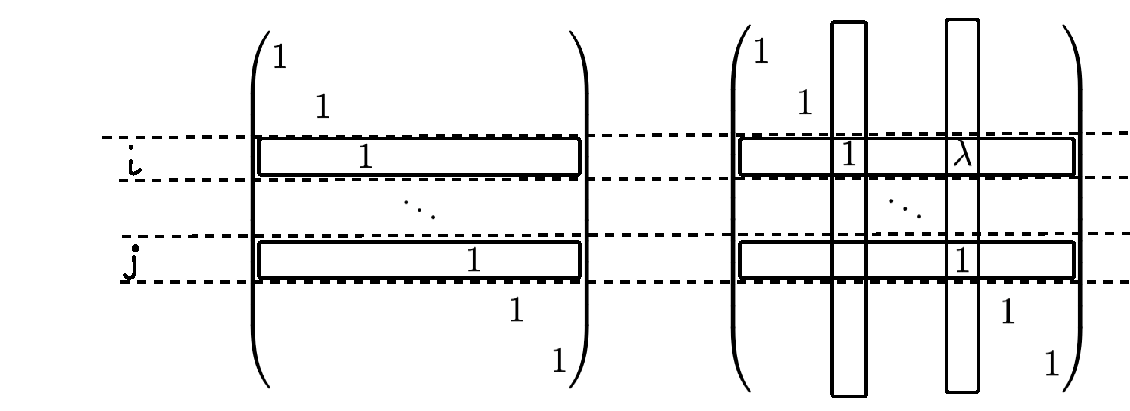
\includegraphics[width=12cm]{image/EP1.pdf}$$
    ЭП2: \tab[6.5cm]:
    $$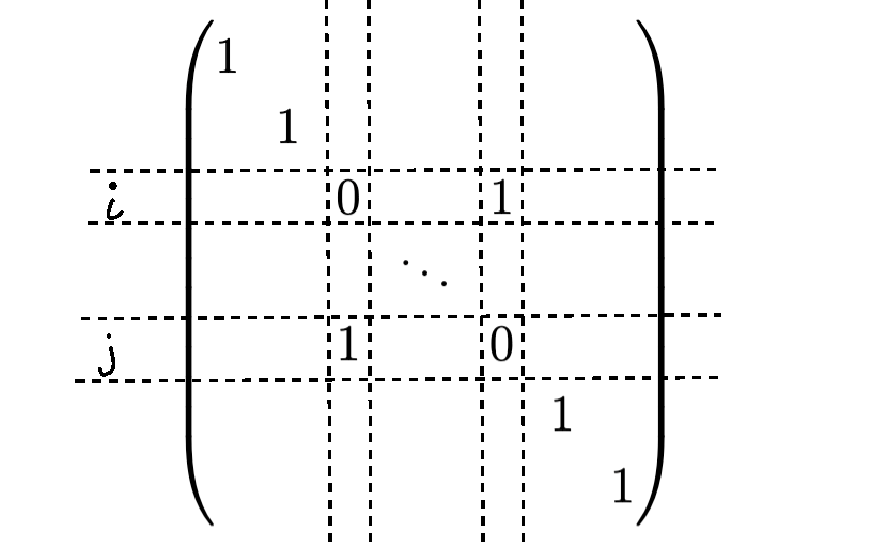
\includegraphics[width=7cm]{image/EP2.pdf}$$
    ЭП3: \tab[5cm] $\begin{pmatrix*}
        1&&&&\\
        &\ddots&&&\\
        &&-1&&\\
        &&&\ddots&\\
        &&&&1
    \end{pmatrix*}$\\
    называются (целочисленными) элементарными матрицами. \\
    (нагло украденными у Славы, пожелайте ему удачно линал пересдать))
\end{definition}
\begin{definition}(ЭП строк целочисленных матриц)
    \begin{itemize}
        \item \textbf{ЭП1}: $\overline{a_i} \to \overline{a_i} + \lambda \overline{a_j}, \ \ i \neq j, k \in \Z$;
        \item \textbf{ЭП2}: $\overline{a_i} \leftrightarrow  \overline{a_j}, \ \ i \neq j$;
        \item \textbf{ЭП3}: $\overline{a_i} \rightarrow (-1) \overline{a_i}$;
    \end{itemize}
\end{definition}
